\documentclass[a4paper, 12pt]{article}

\usepackage{cmap} % make files searchable and copyable
\usepackage{mathtext} % use cyrillic in formulas
\usepackage[T2A]{fontenc} % properly encode fonts
\usepackage[utf8]{inputenc} % properly encode inputs
\usepackage[british]{babel} % multiple languages support

% AMS+ packages for proper mathematical rendering
\usepackage{amsmath}
\usepackage{amsfonts} 
\usepackage{amssymb}
\usepackage{amsthm} 

\usepackage{mathtools}

\usepackage{dsfont} % additional math symbols 
\usepackage{upgreek} % additional upright greek symbols

\usepackage{icomma} % properly set spacing around decimal symbol

\usepackage[shortlabels]{enumitem} % custom list labels

\usepackage{graphicx} % additional image options
\usepackage{pdfpages} % ability to insert pre-made .pdf pages

\usepackage[font=small,labelfont=bf]{caption}
\newcommand{\source}[1]{\caption*{\textbf{Source:} {#1}} }
\usepackage{subcaption} % captions for subfigures 

% joint rows and columns in tables 
\usepackage{multirow}
\usepackage{multicol}

\usepackage{float} % better positioning of objects

\usepackage{listings} % create environment to showcase code

% bibliography stuff
\usepackage{csquotes} 
\usepackage[backend=biber, style=apa, sorting=nty]{biblatex}
\addbibresource{main.bib}

% define geometry of the list
\usepackage{geometry} 
    \geometry{top=20mm}    
    \geometry{bottom=20mm}   
    \geometry{left=20mm}   
    \geometry{right=20mm}  

\usepackage{setspace}
    \onehalfspacing

\usepackage{fancyhdr} % additional controls of headers and footers

\usepackage{hyperref} % hyperreferences and hyperlinks

\usepackage{lipsum}

\usepackage{indentfirst}


\title{IES \LaTeX\ Example}
\author{Ilya Kotelnikov}
\date{\today}

\begin{document}


\includepdf[]{latex_pdf_cover.pdf}

\setcounter{page}{1}

\maketitle

\begin{abstract}
    \lipsum[1-1]
\end{abstract}

\newpage

\tableofcontents

\newpage

\section{How to type text}
When we want to type some text in Latex, we just type it down and it automatically renders in a proper way.

If we want to start a new paragraph, we need to skip a line (press \verb|Enter| twice).

If we want to just start a new line, but not to start a new paragraph, we should use double backslash (\verb|\\|).\\
Like this.

Also there exist command \verb|\newline| that has a similar effect.

It is important to know that the first paragraph in each section (chapter, subsection etc.) is not indented by default and that's why we import \verb|indentfirst| package in the beginning. If you do not want to indent your paragraphs (i.e. all the lines are short and it looks bad when indented) you can comment that line out or just completely remove it.
\section{How to use commands}
All the commands in Latex are used by typing backslash (\verb|\|) and the name of the command right afterwards - for example \verb|\newpage|.

In general the necessary arguments are passed in the curly brackets right after the command itself, like in \verb|\begin{document}| or \verb|\usepackage{multirow}|. 

Sometimes commands can also take additional arguments or some optional parameters. In such cases, they are usually passed in square brackets before the curly ones, for example as in \verb|\usepackage[british]{babel}|.

Commands are usually limited in scope - some commands can be used in the intro to the document, some inside the text, and some only inside the mathmode, that will be discussed later.
\section{How to type formulas}
All the formulas are typed inside mathmode, which renders symbols differently and also allows for the use of special commands/symbols. There are several ways to initiate mathmode environment and they have distinct purposes.

\subsection{Inline mode}
On the basic level formula can be inserted into the paragraph of text by using the dollar sign (\verb|$|). This can be done to write something obvious, e.g. $x+2=5$, or just insert the symbol the same way it appears in the equation - $x$.

\newpage
\subsection{Paragraph mode}
However, long formulas do not look good inside the paragraph, so there are special ways to render them.

\subsubsection{Basic}
\[\sigma^2_t = \omega + \alpha\sigma^2_{t-1}+\beta\varepsilon^2_{t-1}\]

\subsubsection{Variation of advanced}
\begin{equation}
\label{eq:garch_1_1}
    \sigma^2_t = \omega + \alpha\sigma^2_{t-1}+\beta\varepsilon^2_{t-1}
\end{equation}

\subsection{Multiple lines of formulas}

\subsubsection{Multline environment}
\begin{multline}
    1+2+1+1+1+1+\dots+\\
    +8+9+1+1+1+1+\dots+\\
    +12+13+1+1+1+1=11 
\end{multline}

\subsubsection{Align environment}        
\begin{align}
    22+22&=44\\
    3+3&=6
\end{align}

\subsubsection{Equation + aligned}
\begin{equation} 
\label{eq:system}
\begin{aligned}
    \mathbb{E}[r_i]&=r_f+\frac{\mathbb{E}[r_\tau]-r_f}{\sigma_\tau}\sigma_i\\
    \mathbb{E}[r_i]&=r_f+\beta_i(\mathbb{E}[r_M]-r_f)
\end{aligned}
\end{equation}

\subsubsection{Systems of equations}
\[ 
\left\{
    \begin{aligned}
        \mathbb{E}[r_i]&=r_f+\frac{\mathbb{E}[r_\tau]-r_f}{\sigma_\tau}\sigma_i\\
        \mathbb{E}[r_i]&=r_f+\beta_i(\mathbb{E}[r_M]-r_f)
    \end{aligned}
\right.       
\]
        
\[
|x|=
\begin{cases}
    x, &\text{if}\ x \ge 0\\
    -x, &\text{if}\ x<0
\end{cases}
\]

\section{Lists}

\noindent This is an enumerated list:
\begin{enumerate}
    \item First item
    \item Second item
\end{enumerate}

\noindent This is not an enumerated list:
\begin{itemize}
    \item First item
    \item Second item
\end{itemize}

\noindent You can definitely nest lists inside each other:
\begin{enumerate}
    \item Text
    \begin{enumerate}
        \item Text
        \begin{enumerate}
            \item Text
            \item Text
        \end{enumerate}
        \item Text
        \begin{enumerate}
            \item Text
            \item Text
        \end{enumerate}
    \end{enumerate}
    \item Text
    \begin{enumerate}
        \item Text
        \begin{enumerate}
            \item Text
            \item Text
        \end{enumerate}
        \item Text
        \begin{enumerate}
            \item Text
            \item Text
        \end{enumerate}
    \end{enumerate}
\end{enumerate}

\noindent You can manually setup the symbol:
\begin{enumerate}
    \item[a)] Text
    \item[(a] Also text
    \item[(a)] Still text
\end{enumerate}

\noindent You can even change the default iteration (that is using the \verb|enumitem|):
\begin{enumerate}[i.]
    \item Text but with roman enumeration
    \item Also text but with roman enumeration
    \item Still text but with roman enumeration
\end{enumerate}

\section{Tables}
\subsection{Basic Table}
\begin{table}[h]
    \centering
    \label{tab:basic}
    \begin{tabular}{l|cc}
         Row & Greek 1 & Greek 2 \\\hline
         Row 1& $\alpha$ & $\beta$ \\
         Row 2& $\gamma$ & $\theta$
    \end{tabular}
    \caption{Basic Table}
\end{table}

\subsection{Advanced Tables}


\begin{table}[h] \centering 
\label{tab:advanced} 
\begin{tabular}{@{\extracolsep{5pt}}lcc} 
\\[-1.8ex]\hline 
\hline \\[-1.8ex] 
 & \multicolumn{2}{c}{\textit{Dependent variable:}} \\ 
\cline{2-3} 
\\[-1.8ex] & log(-cashflows) & log(c(0.8, 1.1, 1.1, 1.1, 1.3)) \\ 
\\[-1.8ex] & (1) & (2)\\ 
\hline \\[-1.8ex] 
 year & 0.052$^{***}$ &  \\ 
  & (0.004) &  \\ 
  & & \\ 
 c(1, 2, 3, 4, 5) &  & 0.097$^{*}$ \\ 
  &  & (0.032) \\ 
  & & \\ 
 Constant & 3.760$^{***}$ & $-$0.226 \\ 
  & (0.043) & (0.106) \\ 
  & & \\ 
\hline \\[-1.8ex] 
Observations & 20 & 5 \\ 
R$^{2}$ & 0.921 & 0.756 \\ 
Adjusted R$^{2}$ & 0.917 & 0.675 \\ 
Residual Std. Error & 0.093 (df = 18) & 0.101 (df = 3) \\ 
F Statistic & 210.332$^{***}$ (df = 1; 18) & 9.290$^{*}$ (df = 1; 3) \\ 
\hline 
\hline \\[-1.8ex] 
\textit{Note:}  & \multicolumn{2}{r}{$^{*}$p$<$0.1; $^{**}$p$<$0.05; $^{***}$p$<$0.01} \\ 
\end{tabular} 
\caption{Advanced Table} 
\end{table} 

\newpage
\section{Illustrations}

\subsection{Images}

\begin{figure}[h]
    \centering
    
\includegraphics[scale=0.8]{cat_picture.jpeg}
    \caption{Picture of a Strange Cat}
    \label{fig:cat}
\end{figure}

\subsection{Graphs}

\begin{figure}[h]
    \centering
    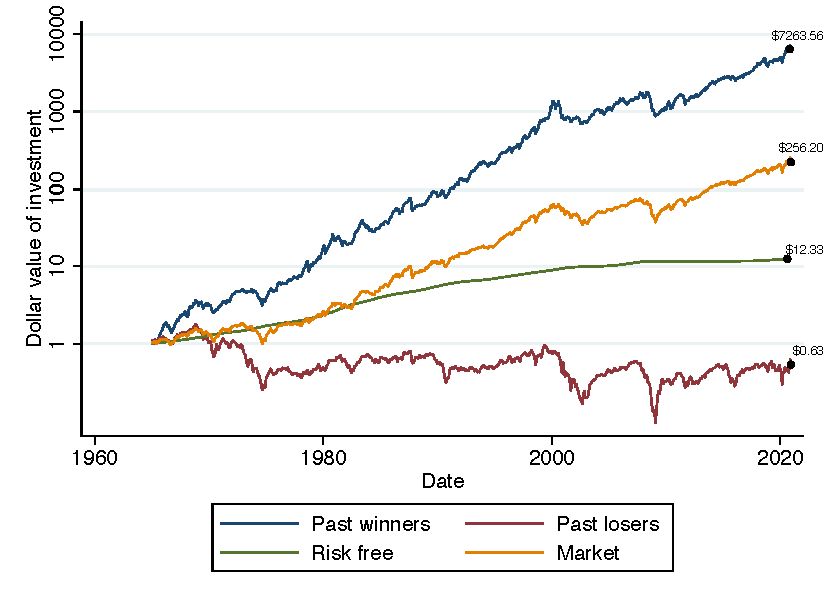
\includegraphics[scale=0.9]{Graph2.pdf}
    \caption{Graph of Different Investment Strategies}
    \label{fig:graph}
\end{figure}

\newpage
\section{Counters and Custom Functions}

\newcounter{problem_number}
\setcounter{problem_number}{0}

\newcommand{\question}[1]{\noindent\addtocounter{problem_number}{1}\textbf{Problem \arabic{problem_number}}\\ #1\\ \\}
    
\question{How many chickens in a bus?}
\question{How many buses in a chicken?}


\nocite{*}
\printbibliography


\end{document}
